%!TEX root = ../template.tex
%%%%%%%%%%%%%%%%%%%%%%%%%%%%%%%%%%%%%%%%%%%%%%%%%%%%%%%%%%%%%%%%%%%%
%% chapter2.tex
%% NOVA thesis document file
%%
%% Chapter with the template manual
%%%%%%%%%%%%%%%%%%%%%%%%%%%%%%%%%%%%%%%%%%%%%%%%%%%%%%%%%%%%%%%%%%%%

\typeout{NT FILE chapter2.tex}

% \printbibliography[heading=subbibliography, segment=\therefsegment, title={\bibname\ for chapter~\thechapter}]
\glsresetall
\chapter{State of the Art}\label{cha:II_SotA}
% escrever aqui qlq coisa de introduçao:

Like any project development, it is always a wise approach studying all the theoretical concepts and current state of the art beforehand. That's the objective of this Chapter;
starting with the clarification of the intricate arrangement of the satellites that constitute a GNSS in section~\ref{sec:II_gnss}, the different positioning techniques inevitably become easier to dissect, through sections~\ref{sec:II_ppp},~\ref{sec:II_rtk},~\ref{sec:II_ppk} and~\ref{sec:II_ntrip}.
Section~\ref{sec:II_battery} then details the battery system of the device, as well as possible solutions to reduce the overall power consumption of this unit (and therefore of the entire equipment).
Finally, the current most relevant solutions (base stations) are addressed and compared, as these will provide helpful guidelines to the development of future beRTK.

% enter a NUTSHELL setting of RTK,
a base station is intended that is capable of fine-tuning the position of the rover (drone);

---------------------

beRTK can be used for:
Enhanced Landing
Surveying fields precisely
Accurate Mapping
Review Work Processes

HEIFU, beRTK and beXStream can be used for:
\begin{itemize}
    \item \textbf{Cartografy and 3D Mapping}
    \item \textbf{Detection and Removal of Asian Wasp hives}
    \item \textbf{Precision Farming}
        a. Survey every inch of your field
            Allows detailed survey of every field
        b. Improves productivity and efficiency 
            Reduce time spent on field-walking
        c. Higher resolution of the field areas of interest 
            It is beneficial for immediate identification and GPS tagging
        d. Earlier identification of potential crop issues
            Use of multispectral sensing technology
    \item \textbf{Search and Rescue}
    \item \textbf{Forest Firing Detection and Monitoring}
    \item \textbf{Border Patrol Monitoring}
    \item \textbf{Demining}
    \item \textbf{Medical Delivery}
    \item \textbf{Infrastructure}
    \item \textbf{High Rise Window Cleaning}
    \item \textbf{Ad hoc Communication Relay}
    \item \textbf{Equipment Monituring in factories}
    \item \textbf{Remote Car Inspection - Insurance}
    \item \textbf{Virtual Traveling}
\end{itemize}
\begin{itemize}
    \item But there is still a great ally for such efficiency, which sometimes goes unnoticed or is even forgotten: Image Processing.

    % Começar com:
    % I. o que é uma base station? fazer analogia
    % II. dizer para que e que serve
    % III. onde/no que é que eu vou empregá-la?
    % IV. que tecnologias utiliza?
    % V. explicar cada tecnologia relativamente a base

    % artigos que li:
    \item a. Experimental Testbed and Methodology for the Assessment of RTK GNSS Receivers Used in Precision Agriculture;

    \item b. DETERMINATION OF THE POSITION USING RECEIVERS INSTALLED IN UAV

    \item c. High-Precision/Throughput Growth Measurement of Crops by Drone with Stereo Matching Based on RTK-GNSS and Single Camera

    \item d. Estimation of the Base Station Position Error in a RTK Receiver Using State Augmentation in a Kalman Filter

    \item e. Resilient Deployment of Drone Base Stations

    \item f. Based on a single-base station RTK control survey and precision analysis 

    \item g. Design of an Autonomous drone for IoT deployment analysis 

    \item h. RTK+ System for Precise Navigation in Shadowed Areas 
\end{itemize}

\section{Global Navigation Satellite System}\label{sec:II_gnss}

Whenever someone wishes to know their current location on Earth, just a few, effortless taps on a smartphone will be the quickest way to do it; this is often associated with the radionavigational system of GPS, which has been around for many years. In a more general manner, this technology can be described as a Global Navigation Satellite System, or GNSS, which refers to any satellite constellation that can be used in order to help navigation throughout the world (as the name suggests).
Therefore, it is possible to conclude that, in order to help tracking their location through the use of satellites, typical smartphones or GPS navigation systems in cars have GNSS receivers, just like a specially designed surveying device.

According to~\cite{novatel_gnss}, the best way to address GNSS receivers as a whole is to start by acknowledging its working basis: satellites. While orbiting the Earth, these machines send out signals that are then acknowledged by receivers (hence the name), helping them calculate their own location on Earth by comparing the received information from other satellites.
This means that a GNSS comprises a network of satellites that continuously orbit the Earth, constantly emitting radiofrequency signals carrying information about their current status, position in space and precise time.
This information is achieved through atomic clocks, installed within the satellite itself. Thus, the process unfolds as follows:

\begin{enumerate}
    \item Satellites will start the transmission of their position in real time;
    \item As this happens, the receiver on Earth will be looking for a signal from the satellite, and by the time that signal is received, there will be a delay between transmission and reception, beign that radio signals travel at the speed of light ($c$);
    \item Knowing both these timestamps, a GNSS receiver is then able to calculate the difference between the two and determine the time it took to receive the signal;
    \item Lastly, multiplying this calculated time interval by the speed of light, it is then possible to find the distance from the satellite to the receiver.
\end{enumerate}
This process is known as ``trilateration'' and is explained in more detail in the following section.

\subsection{Trilateration}\label{sec:II_gnss_trilateration}

Incorporating the idea that the time ($t$) it takes to receive a signal from a satellite multiplied by the speed of light ($c$) will equal the distance ($d$),

\begin{equation}
    d = v\,t = c\,t\,,\medskip
\end{equation}
it indicates that the signal emitted by the satellite propagates in an omnidirectional way, which can be pictured as a sphere around the satellite -- as it's known from radiation and propagation of electromagnetic waves theory --, meaning the signal will reach the Earth in numerous locations (Figure~\ref{fig:omnidirectional}).
Having another satellite orbiting around Earth, the signal emitted by it will reach the surface at some other particular time. Geometrically, this means that the intersection of the spheres that represent these two signals will correspond to a circle, which limits the extensive list of possible solutions -- note that, however, there is still a large amount --, not allowing yet to have an exact location. Adding a third satellite to this scenario will further limit the possible locations of the receiver, narrowing them down to only two points: one in space and another one down on the surface of the Earth. Knowing that a receiver is down on Earth, by using the latter as a fourth surface, the correct location (in a set of $x$, $y$, $z$ coordinates) can be determined.
% meter imagem word: propagação
\begin{figure}[ht]
	\centering
	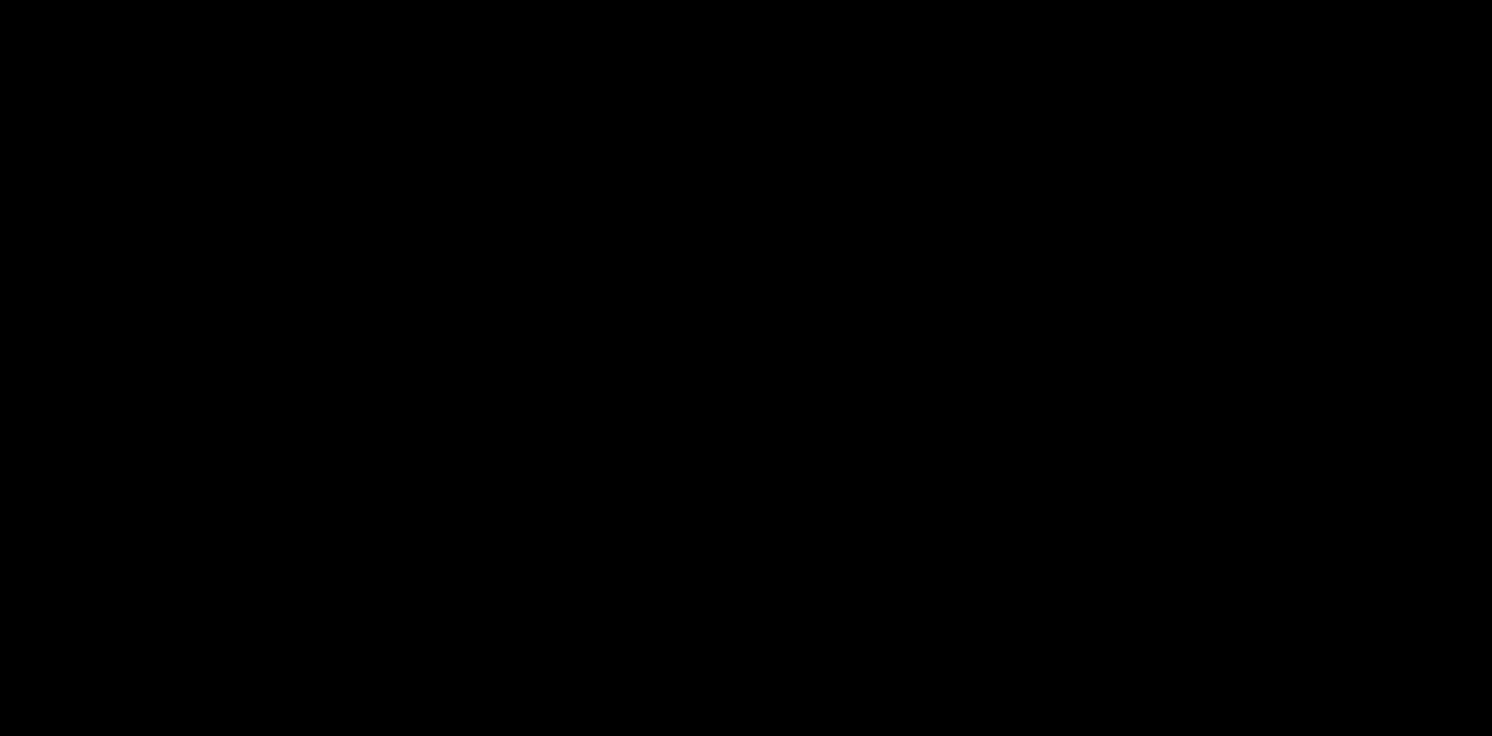
\includegraphics[width=1.0\textwidth]{Chapters/Figures/demo.png}
	\caption{Propagation of satellite signals.}
	\label{fig:omnidirectional}
\end{figure}
However, just three satellites are not enough for an accurate reading, although in theory this process should be enough. The practical use of trilateration must account with a minimum of four satellites in direct line of sight of any point on the surface of the Earth, in order to synchronise the receiver's clock with the satellites', as well as to better the precision of the solution.
There is, nonetheless, one particular phenomenon able to damage the received signal, resulting in less accurate calculations; it is called Dilution of Precision (DOP). This numerical quantity can be measured statistically, while accounting for satellite geometry and location (relative to the receiver) and may, for instance, be impacted by atmospheric or even urban factors.
% meter imagem de predios e sinais afetados
Logically, it is immediately (and rightfully) assumed that the more satellites there are, the higher the positional accuracy will be for the receiver. For that, to achieve a successful observation, three major segments are necessary, known as the space, control and user segments~\cite{gps_USGov,novatel_gnss,ayers_geosystems_2011}, as depicted by Figure~\ref{fig:s_c_u_segment}.

\begin{figure}[ht]
	\centering
	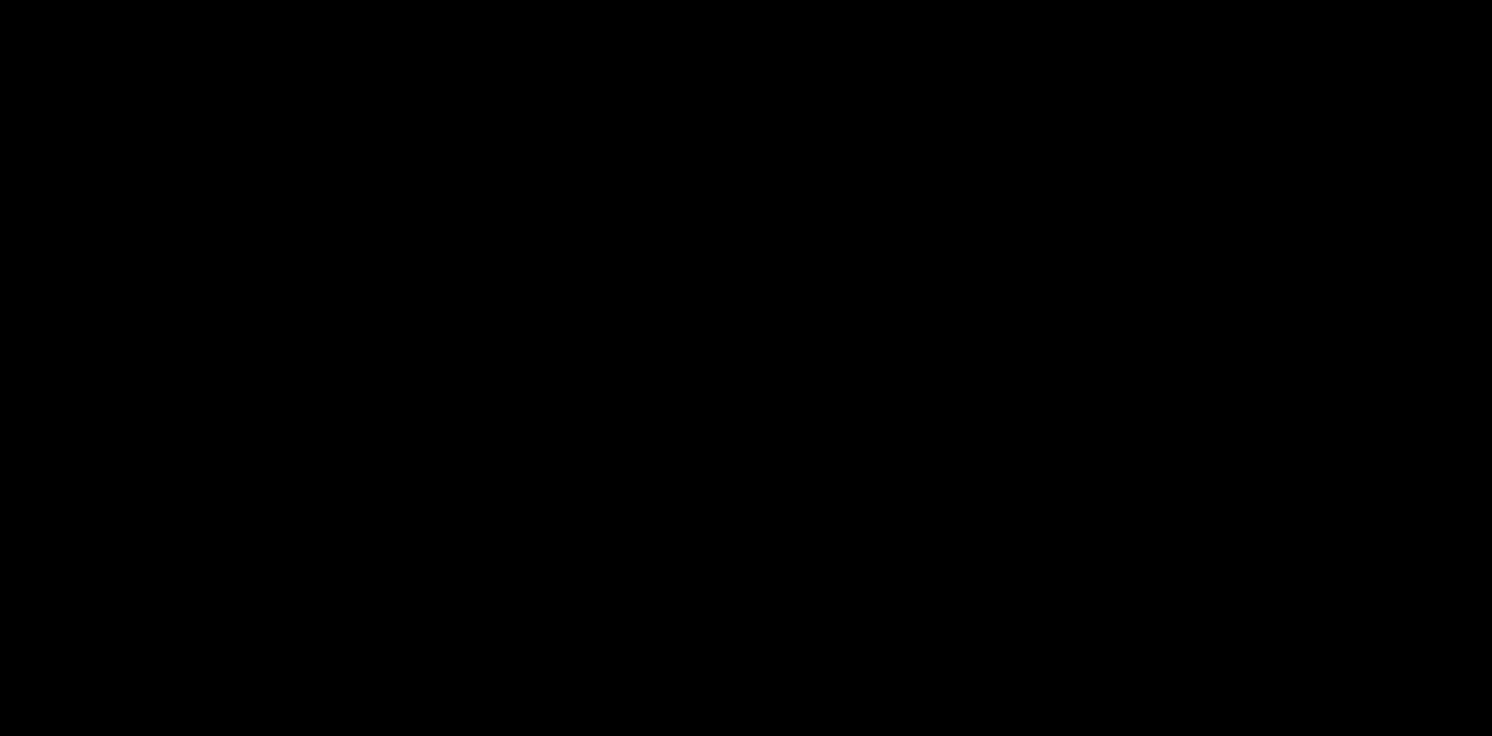
\includegraphics[width=1.0\textwidth]{Chapters/Figures/demo.png}
	\caption{GNSS segments.}
	\label{fig:s_c_u_segment}
\end{figure}

\subsection{Space Segment}\label{sec:II_gnss_space_seg}

The space segment corresponds to the GNSS satellites. All of these follow a certain orbital path thousands of kilometers above the Earth's surface, aiming to assist in the precise location of GNSS-enabled devices on the ground.
Different nations around the world have various satellite networks, with GPS being the most widely known GNSS associated with navigation of all.
% minha parte:
Through~\cite{fed_rad_plan_2008}, it is possible to understand that, in order to enjoy the perks of assisted navigation, the quality behaviour of a GNSS must be ensured. 
A smart approach for that is to analyse the following four performance criteria:

\begin{itemize}
    \item Accuracy: Should not be confused with precision; this parameter acts as a measure of coherence between the estimated (predicted) and actual position of a vehicle, aircraft, or vessel, at any given time;
    \item Availability: In a percentile manner, this gives the navigator the ability to know the amount of time available to benefit from the services provided by the system, within a certain specified coverage area.
    \item Continuity: Refers, in probabilistic terms, to the ability of the entire system of maintaining all required functions, whilst keeping any interruptions out of question. This ensures the operation of the system in a smooth way within a given time interval. All of this assuming that the system was fully available at the start of this operational phase;
    \item Integrity: Measuring the trustworthiness of the information supplied by a navigation system, integrity is also able to consistently issue warnings when navigation through the use of the system is not recommended.
\end{itemize}
All of these parameters are defined as a way to rate the performance of a satellite constellation, which helps tracking down any discrepancies or even problems that might make accurate navigation unacceptable.
Their foundation is known as the Required Navigation Performance (RNP) specification, which characterizes the imperative performance indicators within a defined airspace. By ensuring the proper conduct of a constellation, the perks of a GNSS for navigation purposes are clear.

The development and establishment of the first GNSS ever -- GPS, which was carried out by the United Satates Department of Defense near the end of the 1970s -- relies on a constellation made up of a total of 31 satellites, on which the U.S. Government works to maintain constant operability of a minimum of 24, 95\% of the time, to guarantee global coverage~\cite{gps_USGov}.
Upon its the introduction to civilian use, the desire to cover an even larger portion of the globe only grew, which led to the development of other GNSSs that, together with the already existing GPS, could improve navigational accuracy. Thus, there are currently four global satellite arrangements that make world navigation and precise positioning possible:

% table:-----------------------------
\begingroup
\begin{table}[h]
	\caption{Global satellite positioning systems.}
	\label{tab:5_GNSSs}
	\centering%@{}l@{}@{}c@{}@{}c@{}@{}c@{}@{}c@{}
    % \setlength{\tabcolsep}{10pt} % Default value: 6pt
    % \renewcommand{\arraystretch}{1.5} % Default value: 1
	\begin{tabular}{lcccccc}
        \toprule
        \multicolumn{2}{c}{\multirow{2}*{\textbf{Constellation}}} & \multirow{2}*{\textbf{Satellites}} & \textbf{Orbital} & \textbf{Orbital}     & \textbf{Orbit} \\
        \multicolumn{2}{c}{}                                      &                                    & \textbf{Planes}  & \textbf{Inclination} & \textbf{Radius} \\
        \midrule
     
        \multirow{3}*{
\includegraphics[height=1cm]{Chapters/Figures/flags/usa.png}}&\multirow{3}*{GPS} &  &  &  & \\
        \multirow{3}*{}   &{}             & 27 + 4 (spares) & 6 & 55 degrees & $20,200$ km \\
        \multirow{3}*{}   &{}          & & & & \\

        \midrule

        \multirow{3}*{
\includegraphics[height=1cm]{Chapters/Figures/flags/Russia.png}}&\multirow{3}*{GLONASS} &  &  &  & \\
        \multirow{3}*{}   &{}             & 24 + 3 (spares) & 3 & 64.8 degrees & $19,140$ km \\
        \multirow{3}*{}   &{}          & & & & \\

        \midrule

        \multirow{3}*{
\includegraphics[height=1cm]{Chapters/Figures/flags/Europe.png}}&\multirow{3}*{Galileo} &  &  &  & \\
        \multirow{3}*{}   &{}             & 27 + 3 (spares) & 3 & 56 degrees & $23,222$ km \\
        \multirow{3}*{}   &{}          & & & & \\

        \midrule
        \multirow{3}*{
\includegraphics[height=1cm]{Chapters/Figures/flags/China.png}}&\multirow{3}*{BeiDou} & 5 GEO & --- & --- & $35,787$ km \\
        \multirow{3}*{}   &{}             & 3 IGSO & --- & 55 degrees & $35,787$ km \\
        \multirow{3}*{}   &{}          & 27 MEO & 3 & 55 degrees & $21,525$ km \\
        \bottomrule
    \end{tabular}
\end{table}
\endgroup

%meter/FAZER!!! polygons - imagens das coverages:    !!!!!
% !!!!!!!!!!!!!!!!!!!!!!!!!!!!!!!!!!!!!!!!!!!!!!!!!!!!!!!!

On an additional manner, there are also two extra systems that were developed to provide regional coverage:

\begin{itemize}
    \item NavIC (India): Planned to be made up of seven satellites, this Regional Navigation Satellite System was developed by India to grant regional coverage (hence the (outdated) name IRNSS) to India and its neighbouring area.
    As a result of the launch of the constellation's last satellite in 2016, the IRNSS title was changed to Navigation Indian Constellation (NavIC), by India's Prime Minister Narendra Modi~\cite{navic_news_2016};
    \item QZSS (Japan): Working as another regional navigation satellite system, the development of the Quasi-Zenith Satellite System was accredited by the Japanese Government in order to ensure service to Japan, as well as the Asia-Oceania region and consists of four satellites.
    However, this constellation limits accuracy in its standalone mode, which means it functions as GPS augmentation service\footnote{Augmentation services will be covered in more detail in section~\ref{sec:II_gnss_sbas}.} by synchronisation of clocks use of same frequencies, allowing the use of this system's machinery as extra GPS satellites.
\end{itemize}

Every constellation follows the same purpose of providing services of:

\begin{itemize}
    \item Positioning: Refers to the ability of determining one's location and orientation in an accurate and precise manner, either two-dimensionally or three-dimensionally (whenever necessary), taking a standard reference geodetic system (e.g. World Geodetic System 1984, or WGS84);
    \item Navigation: Enables the determination of the current position, as well as the application of course, orientation and velocity corrections in order to achieve a desired position (relative or absolute) at any location in the world, from subsurface to surface and from surface to space;
    \item Timing: Also encompassing time transfer, timing refers to the ability of acquiring the exact and precise time from a certain standard (in this case Coordinated Universal Time, or UTC), as well as maintain it, anywhere in the world and within timeliness parameters defined by the user.
\end{itemize}
These are known as PNT services~\cite{pnt_2017}.
A good example of the use of this type of data is the GPS system, which is a result of the use of PNT data together with information from maps, as well as from other sources (e.g. meteorological data, traffic, etc.).

Therefore, the space segment essentialy focuses on accurately covering every point on Earth's surface, something which engineers work on to improve everyday, whether it being with precision tweaks to the satellites' atomic clocks or even launching new ones to further complement the existing GNSSs~\cite{euspa_news_2022}. This means that all constellations complement each other, and by being used globally, the location accuracy at any given time is increased.

\subsection{Control Segment}\label{sec:II_gnss_control_seg}

Each satellite's status -- more specifically, its ``health'', position (current and expected), velocity and timing -- is recorded by an internal orbital pattern known as \gls{ephemeris}. Such data is, in turn, included within the transmitted signals. The control segment is found on Earth, at a stationary location, and its control element is used to correct any errors coming from the satellites, being that the more satellites that can be observed in the control segment, the greater the probability of an error to be detected and corrected, thus increasing accuracy in the user segment.

A good example for the control segment is, precisely, a base station: by installing a GNSS receiver at a fixed location, it will continuously collect data from the satellites, as well as any changes or discrepancies in the readings, which can then be corrected later and transferred to the user segment. Nowadays, there are long-term reference stations that are mounted and freely accessible, which eliminates the need for two receivers; having the base and rover together can be too much equipment in some situations and therefore result in larger financial costs.
So, in order to solve this, the rover receiver just needs to be connected to some kind of frame of reference, which will be the control segment used to complete the solution (this could be, for example, an NTRIP network\footnote{NTRIP will be covered in more detail in section~\ref{sec:II_ntrip}.}).
This type of references are generally found in heavily populated areas; anywhere that is more rural or not really connected to society, they may not be available, so the need to have two receivers (base station and rover) in order to complete the three segments will inevitably be felt.

One of the tasks of this segment that is worth mentioning is the constant monitoring of the satellites, i.e. the regular adjustment of trajectory and time information, in order to keep all the transmitted information highly accurate.

\subsection{User Segment}\label{sec:II_gnss_user_seg}

The user segment includes smartphones, rovers and anything that has a GNSS receiver installed; Basically, it is the end result and refers to what needs to be measured (i.e. the location to find). The other two segments act only as a means of helping reach a more precise position for the user segment.
As we try to find the location of a point in a given \gls{geodetic_datum} or coordinate system, regardless of what is being done, taking a survey is about ensuring that all data collected is accurate and any correction elements used are fully understood.

\subsection{Satellite Communication}\label{sec:II_gnss_comm}

It has already been affirmed in section~\ref{sec:II_gnss_trilateration} that GNSS satellites communicate with receivers through radiofrequency signals -- which are electromagnetic signals -- that propagate omnidirectionally. As the name states, these signals rely rigourously on frequency, and that leaves the wonder on how satellite communication actually works.

These machines are designed to continuously orbit along their respective trajectories, and therefore the signals transmitted might run into problems while on their way to Earth, which can occur due to atmospheric reasons or even while the receiver is blocked by something such as a building, for example. An affected signal reaching a recevier will result in a poor reading precision. Table~\ref{tab:GNSS_sys_errors} shows the typical errors intrinsic to the GNSS system.

% no final meter tabela: ATENÇÃO À POSIÇÃO DA TABELA!!
\begingroup
\begin{table}[h]
	\caption{Typical GNSS system errors (adapted from~\cite{novatel_gnss}).}
	\label{tab:GNSS_sys_errors}
	\centering%@{}l@{}@{}c@{}@{}c@{}@{}c@{}@{}c@{}
    % \setlength{\tabcolsep}{10pt} % Default value: 6pt
    % \renewcommand{\arraystretch}{1.5} % Default value: 1
	\begin{tabular}{lc}
        \toprule
        \textbf{Source} & \textbf{Error range} \\
        \midrule     
        Satellite clocks & $\pm 2.0$ m \\
        \midrule
        Orbit errors & $\pm 2.5$ m \\
        \midrule
        Ionospheric delays & $\pm 5.0$ m \\
        \midrule
        Tropospheric delays & $\pm 0.5$ m \\
        \midrule
        Receiver noise & $\pm 0.3$ m \\
        \midrule
        Multipath & $\pm 1.0$ m \\
        \bottomrule
    \end{tabular}
\end{table}
\endgroup

%dizer isto por outras palavras:
The communication process can be characterized through an intricate set of terms such as \gls{pseudorandom}, \gls{correlation} and code division multiple access (CDMA). According to~\cite{novatel_gnss}, GPS is known to be an excellent example capable of clarifying these concepts.
% dar o exemplo de GPS: tem CDMA -> falar de CDMA:
The way GPS satellites communicate through the same frequency bands is through CDMA. This form of spread spectrum enables the modulation of signals via a code defined as being pseudorandom. Receivers know beforehand the code intrinsic to each satellite, which allows synchronisation (correlation) between receivers and that same CDMA code. That way, theoretically, information should be able to flow smoothly, however, due to the aforementioned dilution of precision, signals may be affected while travelling through the atmosphere;
the propagation signal can be affected when it passes through the ionosphere (a layer located roughly 50-1,000 km above Earth's surface) or the troposphere (located about 8-14.5 km above the surface), which correspond to the upper and lower zones of the atmosphere, respectively. These effects depend significantly on frequency, so it is worth noting that signals can be compromised by reflection and even absorption, scintillation, Faraday rotation and \textbf{bandwidth decoherence}~\cite{au_gov_satell}. Considering these problems, GPS was designed to operate in frequencies within the interval of 1 to 2 GHz, which corresponds to a section of the radio spectrum known as the L-band, as represented by Figure~\ref{fig:gps_bands} (which shows the frequncy bands used in GPS communication, known as the L1, L2 and L5 frequencies).
% meter/fazer figura das frequencias do GPS:
\begin{figure}[ht]
	\centering
	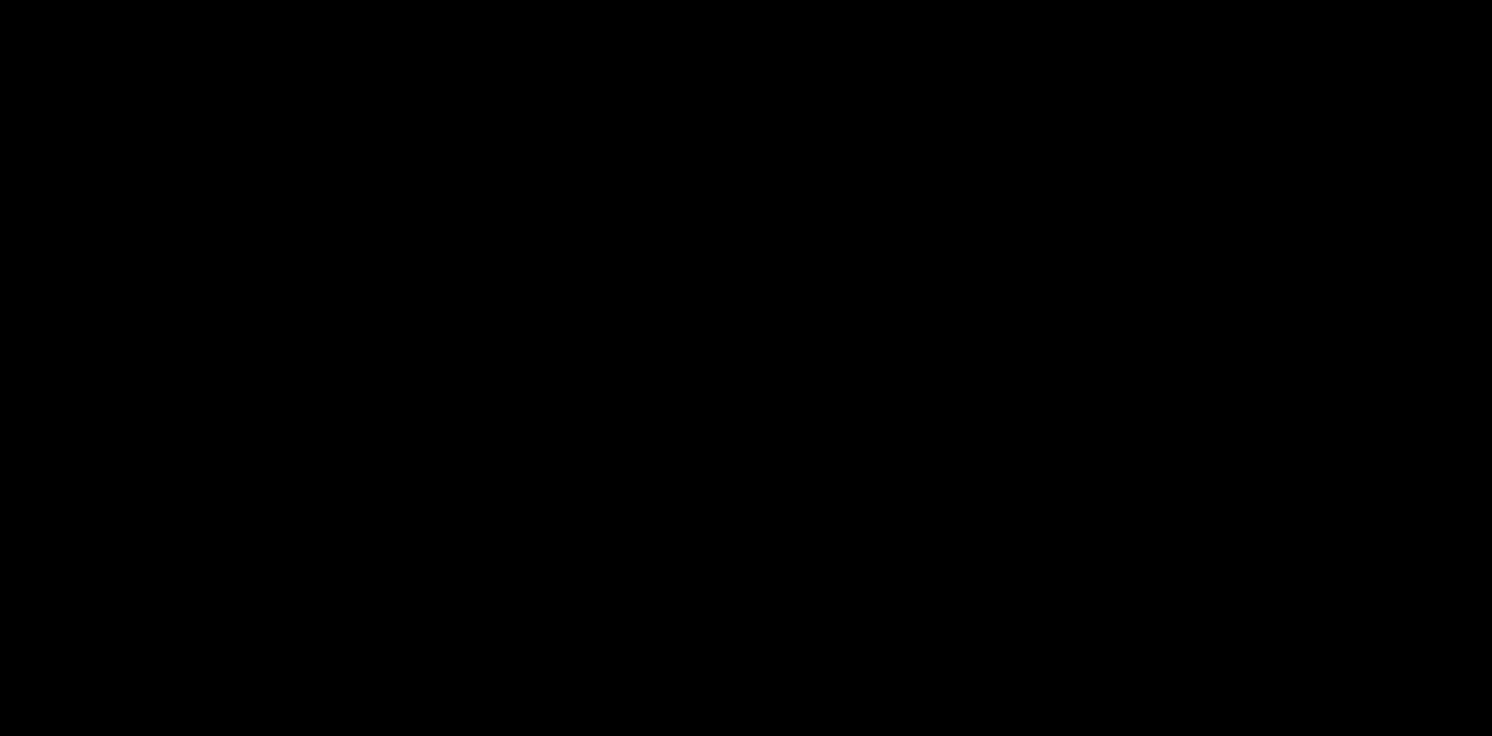
\includegraphics[width=1.0\textwidth]{Chapters/Figures/demo.png}
	\caption{GPS frequency bands.}
	\label{fig:gps_bands}
\end{figure}

This band solves a great part of the stated problems due to its high frequencies, as it 

% razões 1: MUDAR
Simplification of antenna design. If the frequency had been much higher, user antennas may have had to be a bit more complex.
- Ionospheric delay is more significant at lower frequencies.
- Except through a vacuum, the speed of light is lower at lower frequencies
- The coding scheme requires a high bandwidth, which was not available in every frequency band.
- The frequency band was chosen to minimize the effect that weather has on GPS signal propagation.

% razões 2: MUDAR
L1 transmits a navigation message, the coarse acquisition C/A code (freely available to the public) and an encrypted precision (P) code, called the P(Y) code (restricted access). The navigation message is a low bit rate message that includes the following information:
- GPS date and time.
- Satellite status and health. If the satellite is having problems or its orbit is being adjusted, it will not be usable. When this happens, the satellite will transmit the out-of-service message.
- Satellite ephemeris data, which allows the receiver to calculate the satellite's position. This information is accurate to many, many decimal places. Receivers can determine exactly where the satellite was when it transmitted its time.
- Almanac, which contains information and status for all GPS satellites, so receivers know which satellites are available for tracking. On start up, a receiver will recover this "almanac".
The almanac consists of coarse orbit and status information for each satellite in the constellation.

The P(Y) code is for military use.

GPS. The L2 frequency transmits the P(Y) code and, on newer GPS satellites, it also transmits the C/A code (referred to as L2C), providing a second publicly available code to civilian users.

\subsubsection{Signal Propagation}\label{sec:II_gnss_comm_propag}

The layer of the atmosphere that most influences the transmission of GPS (and other GNSS) signals is the ionosphere. These electrons influence electromagnetic wave propagation, including GPS satellite signal broadcasts. Ionospheric delays are frequency dependent so by calculating the range using both L1 and L2, the effect of the ionosphere can be virtually eliminated by the receiver.

The other layer of the atmosphere that influences the transmission of GPS signals is the troposphere. Tropospheric delay is a function of local temperature, pressure and relative humidity. L1 and L2 are equally delayed, so the effect of tropospheric delay cannot be eliminated the way ionospheric delay can be.

Some of the signal energy transmitted by the satellite is reflected on the way to the receiver. This phenomenon is referred to as "multipath propagation". These reflected signals are delayed from the direct signal and, if they are strong enough, can interfere with the desired signal. Techniques have been developed whereby the receiver only considers the earliest-arriving signals and ignores multipath signals.

%meter imagem de sinais de satelite a serem deflected e refleced em predios e tal:
\begin{figure}[ht]
	\centering
	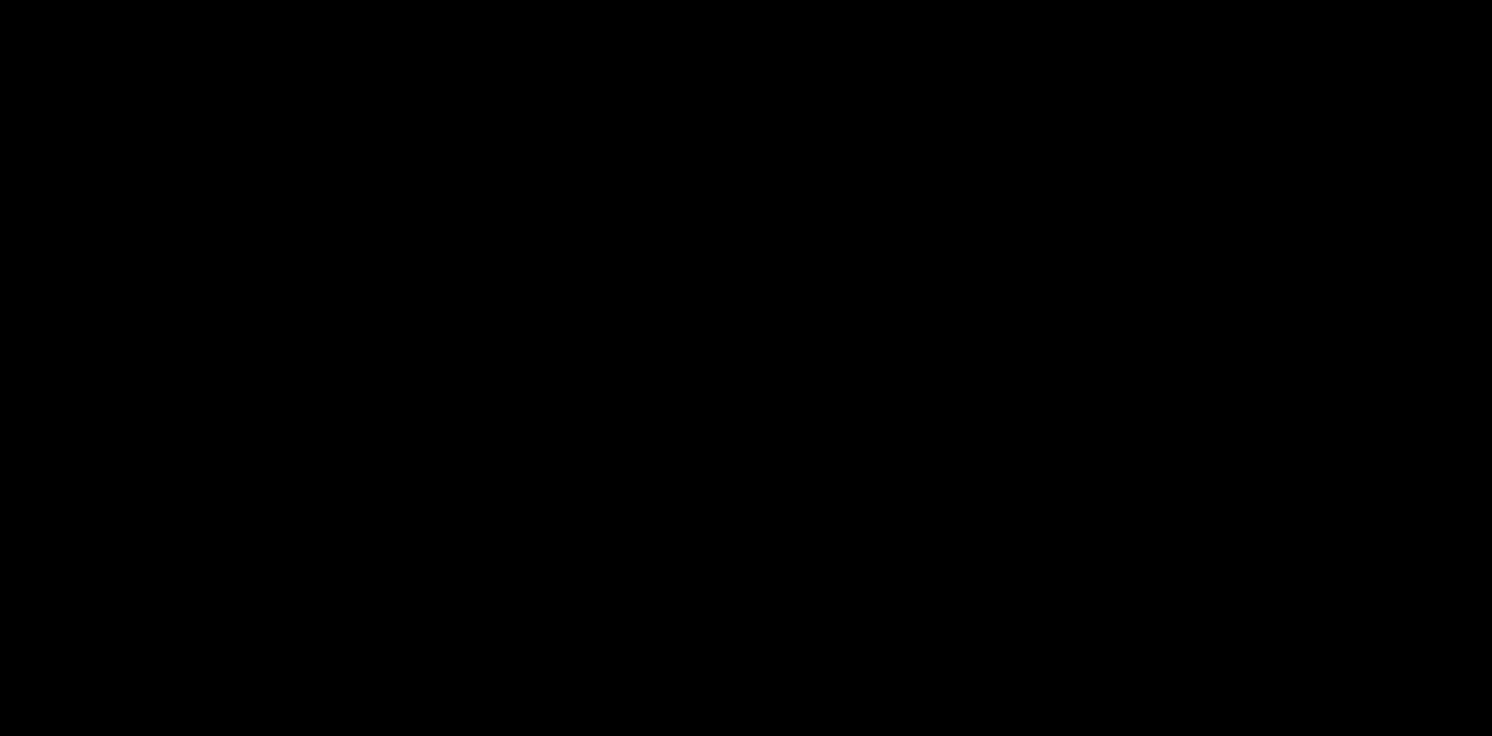
\includegraphics[width=1.0\textwidth]{Chapters/Figures/demo.png}
	\caption{GNSS satellite signal propagation.}
	\label{fig:signals_deflected}
\end{figure}

Upon reception of the signals:
The use of more satellites, if they are available, will improve the position solution;

To determine a fix (position) and time, GNSS receivers need to be able to track at least four satellites. This means there needs to be a line of sight between the receiver's antenna and the four satellites.

Receivers vary in terms of which constellation or constellations they track, and how many satellites they track simultaneously. For each satellite being tracked, the receiver determines the propagation time. It can do this because of the pseudorandom nature of the signals.

Since the receiver knows the pseudorandom code for each satellite, it can determine the time it received the code from a particular satellite. In this way, it can determine the time of propagation.

% fim da parte de propagação.

Important requirement: the requirement of CDMA to operate in a high bandwidth, therefore truly benefiting from this L-band.

It was also specially selected to work on due to the fact that it 

C/A P-code~\cite{ca_p_code_1991}

It is worth stating that the navigation message transmitted is has a low bit rate.

This can explain the reason why these signals should be transmitted in high frequencies, which paves the ground for the next question: Which frequency bands yield the best transmission results for each GNSS?

\subsubsection{Frequency Bands}\label{sec:II_gnss_comm_freq_bands}

% no final meter tabela: ATENÇÃO À POSIÇÃO DA TABELA!!
\begingroup
\begin{table}[h]
	\caption{GNSS signals and frequencies (adapted from~\cite{novatel_gnss}).}
	\label{tab:GNSS_freqs}
	\centering%@{}l@{}@{}c@{}@{}c@{}@{}c@{}@{}c@{}
    % \setlength{\tabcolsep}{10pt} % Default value: 6pt
    % \renewcommand{\arraystretch}{1.5} % Default value: 1
	\begin{tabular}{lcc}
        \toprule

        \textbf{System} & \textbf{Signal} & \textbf{Frequency (MHz)} \\

        \midrule
     
        \multirow{5}*{GPS}      & L1 C/A    & 1575.42 \\
        \multirow{5}*{}         & L1C       & 1575.42 \\
        \multirow{5}*{}         & L2C       & 1227.60 \\
        \multirow{5}*{}         & L2P       & 1227.60 \\
        \multirow{5}*{}         & L5        & 1176.45 \\

        \midrule

        \multirow{4}*{GLONASS}  & L1 C/A    & 1598.0625-1609.3125 \\
        \multirow{4}*{}         & L2C       & 1242.9375-1251.6875 \\
        \multirow{4}*{}         & L2P       & 1242.9375-1251.6875 \\
        \multirow{4}*{}         & L3 OC     & 1202.025            \\
        
        \midrule

        \multirow{5}*{Galileo}  & E1        & 1575.42  \\
        \multirow{5}*{}         & E5a       & 1575.42  \\
        \multirow{5}*{}         & E5b       & 1207.14  \\
        \multirow{5}*{}         & E5 AltBOC & 1191.795 \\
        \multirow{5}*{}         & E6        & 1278.75  \\

        \midrule

        \multirow{6}*{BeiDou}   & B1l       & 1561.098 \\
        \multirow{6}*{}         & B2l       & 1207.14  \\
        \multirow{6}*{}         & B3l       & 1268.52  \\
        \multirow{6}*{}         & B1C       & 1575.42  \\
        \multirow{6}*{}         & B2a       & 1176.45  \\
        \multirow{6}*{}         & B2b       & 1207.14  \\

        \midrule

        NavIC     & L5        & 1176.45 \\

        \midrule

        \multirow{6}*{QZSS}     & L1C/A     & 1575.42 \\
        \multirow{6}*{}         & L1C       & 1575.42 \\
        \multirow{6}*{}         & L1S       & 1575.42 \\
        \multirow{6}*{}         & L2C       & 1227.6  \\
        \multirow{6}*{}         & L5        & 1176.45 \\
        \multirow{6}*{}         & L6        & 1278.75 \\

        \midrule

        \multirow{2}*{SBAS}     & L1        & 1575.42 \\
        \multirow{2}*{}         & L5        & 1176.45 \\

        \bottomrule
    \end{tabular}
\end{table}
\endgroup

%meter imagem das frequencias de todas aonstelações no mesmo referencial: figura 36 novatel_gnss
% meter imagem svg do planeta com todas as GNSS?

%falar de cada frequência: ...
L5:
The United States has implemented a third civil
GPS frequency (L5) at 1176.45 MHz. The modernized
GPS satellites (Block II-F and later) are
transmitting L5.
the modernied benefits of the L5 signal include meeting
the requirements for critical safety-of-life applications
such as that needed for civil aviation
and providing:
- Improved ionospheric correction.
- Signal redundancy.
- Improved signal accuracy.
- Improved interference rejection.

% NOTA FINAL SOBRE GNSS:
As GNSS constellations and satellites are added, we will be able to calculate position more accurately and in more and more places.



\section{GNSS Augmentation}\label{sec:II_gnssAug}

\subsection{Satellite-based Augmentation System (SBAS)}\label{sec:II_gnssAug_sbas}

Used to provide integrity assurance;
Used to increase accuracy and to reduce position errors to less than 1 meter.
"Augmentation of a global navigation satellite system (GNSS) is a method of improving the navigation system's attributes, such as accuracy, reliability, and availability, through the integration of external information into the calculation process."

\subsection{Differential GNSS}\label{sec:II_gnssAug_dgnss}

"Differential" - Aumento infinitamente pequeno de uma quantidade variável.

example: DGPS - Is an enhancement to the Global Positioning System (GPS) which provides improved location accuracy, in the range of operations of each system, from the 15-metre (49 ft) nominal GPS accuracy to about 1-3 centimetres (0.39-1.18 in) in case of the best implementations.
- Differential positioning requires a data link between the base station and rovers, if corrections need to be applied in real-time, and at least four GNSS satellites in view at both the base station and the rovers. The absolute accuracy of the rover's computed position will depend on the absolute accuracy of the base station's position [in pg. 53 of "An Introduction to GNSS, Second Edition"].

8. differential GPS (DGPS) - The term differential GPS, or DGPS, sometimes indicates the application of this technique with coded pseudorange measurements
8.1. relative GPS - usually indicates the application of this technique with carrier phase measurements
8.2. carrier phase measurements
8.3. baselines
in: https://www.e-education.psu.edu/geog862/node/1725

Therefore, by comparing pseudo-range measurements with those made by equipment at a presurveyed location, known as a REFERENCE STATION or BASE STATION, the correlated range errors may be calibrated out, improving the navigation-solution Accuracy! This is the priciple behind Differential GNSS (DGNSS)~\cite{edseee_9101092}. % fazer desenho .svg de base station a "acertar" o drone com os satelites

\subsection{Real-Time Kinematics (RTK)}\label{sec:II_gnssAug_rtk}
\begin{itemize}
    \item % falar de todos os topicos que estejam no doc Word RTK (single- multi-link,...)
    % link da base station ao UAV
    
    %MUDAR, ESTÁ COPIADO!
    So, the difference between RTK and DGPS is that DGPS is the traditional differential GPS.
    RTK is a specific type of DGPS.
    but it uses a newer technology than the traditional DGPS.
    RTK stands for real-time kinematic and commonly uses the RTCM protocol.
    The traditional DGPS uses an older antiquated protocol while RTK uses a newer algorithm, and the protocol is based on RTCM3. 
    %____________
    
    - Used to improve the accuracy of standalone GNSS receivers. Traditional GNSS receivers can only determine the position with na accuracy of about 2-4 meters (?). RTK provides centimeter accuracy.
    - GNSS receiver measure how long it takes for a signal to travel from a satellite to the receiver. Due to the presence of atmosphere between the satellite and the receiver, the transmitted signals are slowed down and are introduced to perturbations. With this in mind, one can immediately assume that transmission times will differ according to the weather at the time of the event. That is the reason why a standalone receiver has a hard time determining its position accurately. RTK is a Technology that solves this issue.
    - 2 receivers are used in RTK. One of them is stationary, the other is a moving rover.
    - Real Time Kinematic (RTK) is a GPS correction technology technique that provides real-time corrections to location data as the drone is surveying and capturing images from a site.    
\end{itemize}

\subsubsection{Frequency Bands}\label{sec:II_gnssAug_rtk_freqbands}
- L1, L2, ... bands

\subsubsection{Initialisation Time}\label{sec:II_gnssAug_rtk_inittime}
- RTK Initialisation Time

\subsubsection{Single-band vs Multi-band}\label{sec:II_gnssAug_rtk_smband}
- Single-band vs Multi-band receiver

\subsubsection{Baseline}\label{sec:II_gnssAug_rtk_baseline}
Baseline in RTK mode and Baseline in PPK mode -- for different projects, a different distance from the rover to the base might be needed. Working near a city is more likely to have base station stations nearby. However, when working in rural areas, base stations are likely to be further away.
Multi-band receivers can work at a longer baseline due to the use of multiple satellite constellations -- as these help in the correction of the readings taken by the base, as mentioned before (earlier?). beRTK can operate with the baseline up to 2.5 km.
fazer uma imagem parecida a esta:
% meter imagem da baseline Emlid

\subsubsection{Accuracy}\label{sec:II_gnssAug_rtk_accuracy}
H: 7 mm + 1 ppm
V: 14 mm + 1 ppm	MEANING OF THIS???
% http://www.apegm.mb.ca/pdf/PD_Papers/GNSSPositioning.pdf
Both single-band and multi-band receivers are capable of centimeter-level absolute accuracy. The main difference is that more factors can influence the stable fix solution in the single-band receiver. Thus, when using a single-band receiver, you can obtain the same absolute accuracy, but only if you have reasonable working conditions.

\subsubsection{PPM}\label{sec:II_gnssAug_rtk_ppm}
PPM expresses a standardized measurement of error -- in millimeters per 1,000 meters -- in relation to orthometric heights. For instance, an orthometric height that has a 2 PPM error rate would indicate an error in measurement equal to 2 millimeters per 1,000 meters traveled. So, if a mountain resort located 1,000 meters inland had a PPM of 2 millimeters, the orthometric height, or elevation, indicated would be accurate to within 2 millimeters.
% https://sciencing.com/difference-between-agl-msl-8524698.html
% https://unstats.un.org/unsd/geoinfo/ungegn/docs/_data_icacourses/_HtmlModules/_Selfstudy/S06/S06_03a.html

\subsubsection{LoRa}\label{sec:II_gnssAug_rtk_LoRa}
``There are number of communication technologies available for interaction between IoT devices today, and the most popular ones are Wi-Fi and Bluetooth. But the problem with Wi-Fi and Bluetooth technology is high power consumption. They also have other limitations like limited range, limited access points etc. ESP8266 module is the most popular Wi-Fi module used in IoT devices, using which we have previously built lot of IoT projects.

Cellular networks also have the same problems of high power consumption and both LAN and Cellular network are quite expensive to cover a wide area. The IoT industries introduced lots of technologies, but none of them was ideal for IoT devices, as they needed to transmit information to long distance without using much power, until the LoRa technology was introduced. LoRa Technology can perform very-long range transmission with low power consumption.

LoRa (Long Range) is a wireless technology that offers long-range, low power, and secure data transmission for M2M (Machine to Machine) and IoT applications. LoRa is a spread spectrum modulation technology that is derived from chirp spread spectrum (CSS) technology. LoRa can be used to connect sensors, gateways, machines, devices, etc. wirelessly. In Europe region, it operates in the 868 MHz band.'' % https://iotdesignpro.com/projects/lora-communication-between-two-arduino-using-LoRa-Module-SX1278

\subsection{Post-Processed Kinematics (PPK)}\label{sec:II_gnssAug_ppk}
PPK is na alternative technique to RTK. With PPK workflow, accurate positioning does not happen in real time, since all algorithms are applied afterwards. Both base station on the ground and rover (usually an UAV) record raw GNSS logs, which are then processed to receive na accurate positioning track.
%meter/fazer imagem do Word:

- PPK is mainly used for UAV mapping.
- Offers a more flexible workflow, allowing to run the processing multiple times using different settings the processing is applied on the logs returned by the both the base station and the rover used on (the?) field.
- PPK allows the inspection of much wider areas, which is why the baseline is greater than the baseline available while working in RTK mode.
- Post Processed Kinematic (PPK) is a GPS correction technology technique that corrects location data after it is collected and uploaded. The data can be uploaded to the cloud for processing or processed using specialise software on your desktop after the flight has been concluded.

\subsection{Precise Point Positioning (PPP)}\label{sec:II_gnssAug_ppp}
- A standalone receiver finds out its position relying on the data obtained from satellites only. Along with raw data from those satellites, the receiver gets navigation messages with satellite clock offset, ionospheric and tropospheric corrections (atmospheric-related disturbances), etc. Due to information about these offsets, the receiver may calculate its position with a few meters' accuracy. If there were (was) no navigation data, the accuracy would be much worse.
- In RTK and PPK, these offsets might be eliminated since both (the) base station and the rover operate in quite similar conditions.
- PPP allows the single receiver (rover) to achieve high-level accuracy without the use of corrections from the base station.
- To calculate the coordinates, PPP uses the same data that is provided by the navigation message but much more accurate. Thereby, the single receiver (rover) might determine its position with a centimetre-level accuracy using only raw data and precise ephemerides and clock offsets provided by a PPP service.
- The PPP technique is commonly used for determining the absolute base position for further RTK/PPK surveys.

%

\subsection{NTRIP}\label{sec:II_ntrip}

%daniel:
As stated in section~\ref{sec:II_gnss_comm}, if a receiver relies solely on satellite signals for positioning, the rate at wich information will be received will be rather low. A great way to bypass such (problem) is to rely on internet connection to get position corrections. A great example of this is the Network Transport of RTCM via Internet Protocol, or NTRIP.

% falar de todos os topicos que estejam no doc Word NTRIP
The fact that beRTK is connected to the NTRIP network allows you to start with a more precise idea of its location and therefore faster convergence.
"Real Time Kinematic technique requires 2 receivers. One of them is stationary and is called "base station", the other one is "rover". The base station measures errors, and knowing that it is stationary transmits corrections to the rover (refer to How RTK works for more information about RTK). Sometimes CORS and NTRIP networks take the place of traditional base stations. They provide accurate absolute position and send corrections over the Internet. Typically the distance between the reference station and local rover shouldn't exceed 10-15 km due to the ionospheric effect. So if the reference station is located too far or simply is absent in the area you will need a local base station. Other advantages of your own base are independence from the Internet connection and lack of NTRIP subscription fees."

- If the accurate absolute position of the base has been determined only after the job has been done, the offset of the map can be determined and corrected.

----------------
% https://www.youtube.com/watch?v=uytd48Vb-fs&ab_channel=RamiTamimi
"NTRIP (Network Transport of RTCM via Internet Protocol) and CORS (Continuously Operating Reference Station) are forms of RTK differential correction that are done using a cellular modem and base station network."
"how to obtain high accuracy positioning utilising just one GNSS recevier?
As described in section (\textbf{ref}) , it is possible obtain high accuracy positioning by setting up two GNSS receivers, which will act as a base station and a rover. Therefore, this method requires double the cost of the method presented in this section. There is a way to use only one GNSS receiver and have RTK-enabled positioning, through the use of a CORS (Continuously Operating Reference System) network. These stations are permanentely set up on a single known location, and continue to observe satellites and perform corrections based on any errors that they observe. Most municipalities, states and countries own these systems and allow public access to anyone that sets up na account. CORS stations are used by geodesists in order to measure any changes that happen on the Earth's surface, and using the same position that they are in, can also help geodesist measures earthquakes, volcanic eruptions or any tectonic movement (the latter can be concluded due to the fact that, in Portugal's network of CORS stations (ReNEP), the information available online also displays the tectonic plate on which the particular station is located.) -- this means that CORS stations can be used as the control segment for rover positioning."


NTRIP network -- The Network Transport of RTCM via Internet Protocol is, as the name suggests, a process able to be performed through the internet.

If there are no NTRIP stations within a radius of (?) from the intended mission site, a base station will need to be used in order to obtain the precise positioning through RTK, i.e. through the methodology described in section (\textbf{ref}).
"it is very fast to obtain a fix. Rather than utilising our own base station for the corrections, the public NTRIP network is used, and the receiver (rover) will be connected to a base station in that network."
Fazer uma imagem parecida a esta: % ver Word

An internet based application that makes the RTCM Correction data from the CORS stations available to anyone with an internet connection and the appropriate log on credentials to the NTRIP server. Typically uses a mobile link to get to the internet and the NTRIP server. % https://www.teejet.com/CMSImages/TEEJET/documents/technical-updates/98-01410%20r0%20en%20tech%20update%20ntrip%20rx610.pdf



% \section{Battery System}\label{sec:II_battery}
% % falar de todos os topicos que estejam no doc Word Battery

% The formula is (Wh)/(h) = (W). For example, if you have 100 Wh for a duration of 2 hours, then the wattage is (100)/(2) = (50) Watts.
% (Watthours is a measure of energy and watts is a unit of power. Power multiplied by time is enery).

% como cada uma das baterias atualmente em uso is rated for (as?) 7.4V, 1070 mAh, that corresponds to 7.918 Wh.

% % LiFePO$_4$ better than Li-ion batteries?
% ``The LiFePO$_4$ battery has the edge over lithium-ion, both in terms of cycle life (it lasts 4-5x longer), and safety. This is a key advantage because lithium ion batteries can overheat and even catch fire, while LiFePO4 does not''% citation needed

% \subsection{USB Type-C}\label{sec:II_usb_c}
% % ler wiki do USB-C e derivar os topicos daí
% % depois ir ao IEEEXplore procurar papers que dêem backup

% \subsubsection{Power Delivery}\label{sec:II_usb_c_PD}
% % PD is a protocol

\section{Current Solutions}\label{sec:II_curr_solutions}
It is necessary to adapt all the solutions abordadas to the current software component; this means that all the solutions have to be implemented.

16. explicar o que cada célula do excel significa, tanto as que considerei mais importantes como as outras

% gravar como pdf/imagem; meter no corpo do texto
% na versao final a tabela sera feita completamente em latex
